% sips -s format png your_pdf_file.pdf --out your_png_file.png

\documentclass[tikz,border=1mm]{standalone}

\usepackage{amsmath}
\usepackage{graphicx}
\renewcommand\familydefault{\sfdefault} 
\usepackage[T1]{fontenc}

\usetikzlibrary{arrows,shapes,calc,math,decorations.fractals,patterns,backgrounds,decorations.markings}
\tikzset{every picture/.style={/utils/exec={\sffamily}}}
\tikzset{point/.style={fill,circle,inner sep=1.5pt}}
\tikzset{vector/.style={-triangle 45, blue, line width=1pt}}
\tikzset{dblarrow/.style={<->}}
\tikzset{axis/.style={-stealth', line width=1pt}}

\renewcommand{\vec}{\mathbf}

\begin{document}

% R3
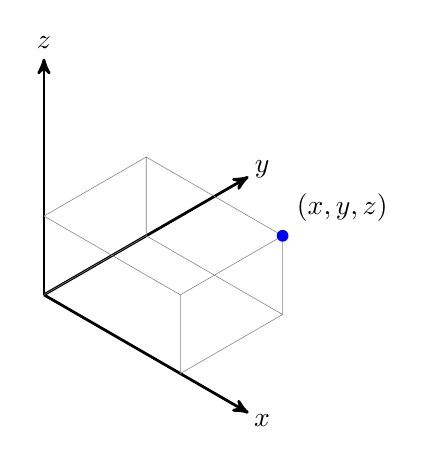
\begin{tikzpicture}
    \tikzmath{\x=-30;\y=-\x;\z=90;\al=3;\lx=2;\ly=1.5;\lz=1;}
    \draw [axis] (0,0) -- ++(\x:\al) node at (\x:\al+0.2) {$x$};
    \draw [axis] (0,0) -- ++(\y:\al) node at (\y:\al+0.2) {$y$};
    \draw [axis] (0,0) -- ++(\z:\al) node at (\z:\al+0.2) {$z$};
    \draw [help lines] (\x:\lx) -- ++(\y:\ly) -- ++(\x+180:\lx) -- ++(\y+180:\ly)
        (\z:\lz) -- ++(\x:\lx) -- ++(\y:\ly) -- ++(\x+180:\lx) -- ++(\y+180:\ly)
        (\x:\lx) -- ++(\z:\lz) (\y:\ly) -- ++(\z:\lz) ($(\x:\lx)+(\y:\ly)$) -- ++(\z:\lz) coordinate (1);
    \node [point,blue,label={45:$(x,y,z)$}] at (1) {};
\end{tikzpicture}

% Vector
% \begin{tikzpicture}
%     \node [point,label={180:$A$}] (1) at (0, 0) {};
%     \node [point,label={0:$B$}] (2) at (30:3) {};
%     \draw [vector] (1) -- node [above left] {$B - A$} (2);
% \end{tikzpicture}

% R3 vector
% \begin{tikzpicture}
%     \tikzmath{\x=-30;\y=-\x;\z=90;\al=2;\lx=2;\ly=2;\lz=1;}
%     \draw [axis] (0,0) -- ++(\x:\al) node at (\x:\al+0.2) {$x$};
%     \draw [axis] (0,0) -- ++(\y:\al) node at (\y:\al+0.2) {$y$};
%     \draw [axis] (0,0) -- ++(\z:\al) node at (\z:\al+0.2) {$z$};
%     \coordinate (1) at (0:3);
%     \coordinate (2) at ($(1)+(\x:\lx)$);
%     \coordinate (3) at ($(2)+(\y:\ly)$);
%     \coordinate (4) at ($(1)+(\y:\ly)$);
%     \coordinate (5) at ($(1)+(\z:\lz)$);
%     \coordinate (6) at ($(2)+(\z:\lz)$);
%     \coordinate (7) at ($(3)+(\z:\lz)$);
%     \coordinate (8) at ($(4)+(\z:\lz)$);
%     \draw [vector] (1) -- node [above left] {$\vec{a}$} (7);
%     \draw [<->] ($(1)+(\x-90:0.2)$) -- node [below] {$a_1$} ++(\x:\lx);
%     \draw [<->] ($(1)+(\x:\lx)+(\y-90:0.2)$) -- node [below right] {$a_2$} ++(\y:\ly);
%     \draw [<->] ($(1)+(\x:2)+(\y:\ly)+(0:0.2)$) -- node [right] {$a_3$} ++(\z:\lz);
%     \draw [help lines] (1) -- (2) -- (3) -- (4) -- (1) 
%         (5) -- (6) -- (7) -- (8) -- (5)
%         (1) -- (5) (2) -- (6) (3) -- (7) (4) -- (8);
% \end{tikzpicture}

% Vector example
% \begin{tikzpicture}
%     \draw [help lines] (0,0) grid (6, 4);
%     \draw [axis] (0,0) -- (0:6.5) node at (0:6.7) {$x$};
%     \draw [axis] (90:0) -- (90:4.5) node at (90:4.7) {$y$};
%     \node [point,label=below left:$A$] (1) at (1,1) {};
%     \node [point,label=above right:$B$] (2) at (5,3) {};
%     \draw [vector] (1) to (2);
%     \foreach \i in {0,...,6} {
%         \node [below] at (\i,0) {$\i$};
%     }
%     \foreach \i in {0,...,4} {
%         \node [left] at (0,\i) {$\i$};
%     }
% \end{tikzpicture}

% % Position vector
% \begin{tikzpicture}
%     \tikzmath{\x=-30;\y=-\x;\z=90;\al=2;\lx=2;\ly=2;\lz=1;}
%     \draw [axis] (0,0) -- ++(\x:\al) node at (\x:\al+0.2) {$x$};
%     \draw [axis] (0,0) -- ++(\y:\al) node at (\y:\al+0.2) {$y$};
%     \draw [axis] (0,0) -- ++(\z:\al) node at (\z:\al+0.2) {$z$};
%     \node [below left] at (0, 0) (O) {$(0,0,0)$};
%     \node [point,label=right:{$(x,y,z)$}] at (15:4) (P) {};
%     \draw [vector]  (0, 0) --  (P) node [pos=0.5,below right] {$\vec{p}$};
% \end{tikzpicture}

% Vector magnitude
% \begin{tikzpicture}
%     \draw [vector] (0,0) -- ++(20:4) node [pos=0.5,above] {$\vec{a}$};
%     \draw [<->] ($(0,0)+(-70:0.5)$) -- ++(20:4) node [pos=0.5,below,rotate=20] {$\|\vec{a}\|$};
% \end{tikzpicture}

% % Vector equality
% \begin{tikzpicture}
%     \tikzmath{\x=0;\y=90;}
%     \draw [axis] (0,0) -- ++(\x:7) node at (\x:7+0.2) {$x$};
%     \draw [axis] (0,0) -- ++(\y:4) node at (\y:4+0.2) {$y$};
%     \draw [vector] (1, 1) -- node [above left] {$\vec{a}$} ++(1,1);
%     \draw [vector, red] (3, 2) -- node [above left] {$\vec{b}$} ++(1,1);
%     \draw [vector, green!75!black] (3, 1.5) -- node [above left] {$\vec{c}$} ++(-1,-1);
%     \draw [vector, black] (4, 1) -- node [above left] {$\vec{d}$} ++(2,2);
%   \end{tikzpicture}


% Vector addition
% \begin{tikzpicture}
%     \draw [axis] (0,0) -- (6,0) node [right] {$x$};
%     \draw [axis] (0,0) -- (0,5) node [above] {$y$};
%     \coordinate (1) at (1, 1);
%     \coordinate (2) at (2, 3);
%     \coordinate (3) at (4, 2);
%     \coordinate (4) at (5, 4);
%     \draw [vector] (1) -- node [above left] {$\vec{a}$} (2);
%     \draw [vector, red] (2) -- node [above left] {$\vec{b}$} (4);
%     \draw [vector, red] (1) -- node [below right] {$\vec{b}$} (3);
%     \draw [vector] (3) -- node [below right] {$\vec{a}$} (4);
%     \draw [vector, green!75!black] (1) -- node [above,rotate=36.87] {$\vec{a}+\vec{b}$} (4);
%     \draw [help lines,dashed] (-1, 1) -- (1) -- (1, -1);
%     \draw [help lines,dashed] (-0.5, 3) -- (2) -- (2, -0.5);
%     \draw [help lines,dashed] (-1, 4) -- (4) -- (5, -1);
%     \draw [<->,blue] (1, -0.2) -- node [below] {$a_1$} ++(1, 0);
%     \draw [<->,red] (2, -0.2) -- node [below] {$b_1$} ++(3, 0);
%     \draw [<->,green!75!black] (1, -0.8) -- node [below] {$a_1+b_1$} ++(4, 0);
%     \draw [<->,blue] (-0.2, 1) -- node [left] {$a_2$} ++(0, 2);
%     \draw [<->,red] (-0.2, 3) -- node [left] {$b_2$} ++(0, 1);
%     \draw [<->,green!75!black] (-0.8, 1) -- node [above,rotate=90] {$a_2+b_2$} ++(0, 3);
% \end{tikzpicture}

% Scalar multiplication of a vector
% \begin{tikzpicture}
%     \draw [vector] (0, 0) -- node [above left] {$\vec{a}$} ++(45:2);
%     \draw [vector,red] ($(2, 0)+(45:2)$) -- node [above left] {$-\vec{a}$} ++(225:2);
%     \draw [vector,green!75!black] (4, 0) -- node [above left] {$\frac{1}{2}\vec{a}$} ++(45:1);
%     \draw [vector,black] (6, 0) -- node [above left] {$2\vec{a}$} ++(45:4);
%     \draw [vector,cyan] ($(8, 0)+(45:1)$) -- node [above left] {$-\frac{1}{2}\vec{a}$} ++(225:1);
% \end{tikzpicture}

% Dot product
% \begin{tikzpicture}
%     \draw [vector] (0, 0) -- node [below] {$\vec{a}$} ++(0:3);
%     \draw [vector, red] (0, 0) -- node [above left] {$\vec{b}$} ++(45:3);
%     \draw (0:1) arc (0:45:1);
%     \node at (22.5:0.67) {$\theta$};
% \end{tikzpicture}

% % Cross product
% \begin{tikzpicture}
%     \tikzmath{\a=-30;\b=-\a;\axb=90;\bxa=\axb+180;}
%     \draw [vector] (0,0) -- (\a:2) node [pos=0.75,below left] {$\vec{a}$} ;
%     \draw [vector, red] (0,0) -- (\b:2) node [pos=0.75,above left] {$\vec{b}$};
%     \draw [vector, green!75!black] (0, 0) -- node [left] {$\vec{a}\times \vec{b}$} ++(\axb:2);
%     % \draw [vector, black] (0, 0) -- node [left] {$\vec{b}\times \vec{a}$} ++(\bxa:1.5);
%     \draw (\a:0.3) -- ++(90:0.3) -- ++(\a:-0.3);
%     \draw (\b:0.3) -- ++(90:0.3) -- ++(\b:-0.3);
% \end{tikzpicture}

% Basis vectors
% \begin{tikzpicture}
%     \tikzmath{\x=-30;\y=-\x;\z=90;\al=3;\lx=1.5;\ly=1;\lz=2;}
%     \draw [axis] (0,0) -- ++(\x:\al) node at (\x:\al+0.2) {$x$};
%     \draw [axis] (0,0) -- ++(\y:\al) node at (\y:\al+0.2) {$y$};
%     \draw [axis] (0,0) -- ++(\z:\al) node at (\z:\al+0.2) {$z$};
%     \coordinate (1) at (0,0);    
%     \coordinate (2) at (0,0);
%     \coordinate (3) at (0,0);
%     \draw [vector, red, line width=1pt] (1) -- ++(\x:2) node [pos=0.5,below] {$\vec{i}$};
%     \draw [vector, green!75!black, line width=1pt] (2) -- ++(\y:2) node [pos=0.5, above] {$\vec{j}$};
%     \draw [vector, blue, line width=1pt] (3) -- ++(\z:2) node [pos=0.5,left] {$\vec{k}$};
% \end{tikzpicture}

% Vector equation of a line
% \begin{tikzpicture}
%     \tikzmath{\x=30;\y=-\x;\z=90;\al=2;}
%     \coordinate (P) at (4, 1);
%     \draw [axis] (0,0) -- ++(\x:\al) node at ++(\x:0.2) {$x$};
%     \draw [axis] (0,0) -- ++(\y:\al) node at ++(\y:0.2) {$y$};
%     \draw [axis] (0,0) -- ++(\z:\al) node at ++(\z:0.2) {$z$};
%     \draw [line width=1pt] ($(P)+(200:3)$) -- ++(20:8) node [right] {$\ell$};
%     \node [point,blue,label={270:$\vec{p}$}] (P) at (P) {};
%     \node [point,red,label={315:\color{red}$\vec{p}+\vec{d}$}] (P1) at ($(P)+(20:2)$) {};
%     \node [point,red,label={315:\color{red}$\vec{p}+2\vec{d}$}] at ($(P)+(20:4)$) {};
%     \node [point,red,label={315:\color{red}$\vec{p}-\vec{d}$}] at ($(P)+(200:2)$) {};
%     \draw [vector,blue,line width=1pt] (P) --  (P1) node [pos=0.5,below] {$\vec{d}$};
% \end{tikzpicture}

% Intersecting lines
% \begin{tikzpicture}
%     \tikzmath{\x=-30;\y=-\x;\z=90;\a1=30;\a2=140;}
%     \draw [axis] (0,0) -- ++(\x:2) node at ++(\x:0.2) {$x$};
%     \draw [axis] (0,0) -- ++(\y:2) node at ++(\y:0.2) {$y$};
%     \draw [axis] (0,0) -- ++(\z:2) node at ++(\z:0.2) {$z$};
%     \coordinate (P) at (3,1);
%     \coordinate (Q) at ($(P)+(3,0)+(\a2:-1)$);
%     \draw [line width=1pt] ($(P)+(\a1:-1)$) -- ++(\a1:4) node [pos=0, below left] {$\ell_1$};
%     \draw [line width=1pt] ($(Q)+(\a2:-1)$) -- ++(\a2:4) node [pos=0, below right] {$\ell_2$};
%     \draw [vector] (P) -- node [above left] {$\vec{d}_1$} ++(\a1:1.5);
%     \draw [vector, red] (Q) -- node [above right] {$\vec{d}_2$} ++(\a2:1.5);
%     \node [point,blue,label={below right:\textcolor{blue}{$\vec{p}_1$}}] at (P) {};
%     \node [point,red,label={below left:\textcolor{red}{$\vec{p}_2$}}] at (Q) {};
%     \node (point) [point] at ($(P)+(\a1:2.05)$) {};
%     \node (label) at ($(point)+(2,0)$) {intersection};
%     \draw [->,shorten >= 4pt] (label) -- (point);
% \end{tikzpicture}

% Parallel lines
% \begin{tikzpicture}
%     \tikzmath{\x=-30;\y=-\x;\z=90;\a1=30;}
%     \draw [axis] (0,0) -- ++(\x:2) node at ++(\x:0.2) {$x$};
%     \draw [axis] (0,0) -- ++(\y:2) node at ++(\y:0.2) {$y$};
%     \draw [axis] (0,0) -- ++(\z:2) node at ++(\z:0.2) {$z$};
%     \coordinate (P) at (3,0.5);
%     \coordinate (Q) at ($(P)+(3,0)$);
%     \draw ($(P)+(\a1:-1)$) -- ++(\a1:4) node [right] {$\ell_1$};
%     \draw ($(Q)+(\a1:-1)$) -- ++(\a1:4) node [right] {$\ell_2$};
%     \draw [vector] (P) -- node [above left] {$\vec{d}_1$} ++(\a1:1);
%     \draw [vector, red] (Q) -- node [below right] {$\vec{d}_2=k\vec{d}_1$} ++(\a1:2);
% \end{tikzpicture}

% Skew lines
% \begin{tikzpicture}
%     \tikzmath{\x=-30;\y=-\x;\z=90;\al=3;}
%     \coordinate (O1) at (0,0);
%     \coordinate (O2) at (\y:3.5);
%     \filldraw [draw=red,fill=red!20,opacity=0.5] ($(O1)+(\x:-2)+(\z:-2)$) -- ++(\x:4) -- ++(\z:4) -- ++(\x:-4) -- ++(\z:-4);
%     \filldraw [draw=green, fill=green!20, opacity=0.5] ($(O2)+(\x:-2)+(\z:-2)$) -- ++(\x:4) -- ++(\z:4) -- ++(\x:-4) -- ++(\z:-4);
%     \draw [axis] (\x:-\al) -- (\x:\al) node at ++(\x:0.2) {$x$};
%     \draw [axis] (0,0) -- (\y:3.5) node at ++(\y:0.2) {$y$};
%     \draw [axis] (\z:-\al) -- (\z:\al) node at ++(\z:0.2) {$z$};
%     \draw [thick,red] ($(O1)+(\x:-2)+(\z:-1)$) -- ($(O1)+(\x:1)+(\z:2)$) node [left,pos=0,black] {$\ell_1$};
%     \draw [thick,green] ($(O2)+(\x:-2)+(\z:1)$) -- ($(O2)+(\x:1)+(\z:-2)$) node [left,pos=0,black] {$\ell_2$};
% \end{tikzpicture}

% Planes
% \begin{tikzpicture}
%     \tikzmath{\a1=330;\a2=30;\l1=4;\l2=4;}
%     \fill [gray!50,opacity=0.5] (0,0) -- ++(\a1:\l1) -- ++(\a2:\l2) -- ++(\a1+180:\l1) -- cycle;
%     \node [point,label={90:$\vec{p}$}] at ($(\a1:1)+(\a2:1)$) (P) {};
%     \node [point,label={0:$\vec{r}$}] at ($(\a1:3)+(\a2:3)$) (Q) {};
%     \draw [vector] (P) -- node [below left] {$t_1 \vec{d}_1$} ++(\a1:2);
%     \draw [vector, red] ($(P)+(\a1:2)$) -- node [below right] {$t_2 \vec{d}_2$} (Q);
% \end{tikzpicture}

% Normal vector
% \begin{tikzpicture}
%     \tikzmath{\x=-15;\y=45;\z=90;\l1=4;\l2=4;}
%     \fill [gray!50,opacity=0.5] ($(0,0)+(\x:-1.5)+(\y:-1.5)$) -- ++(\x:5) -- ++(\y:4) -- ++(\x:-5) -- ++(\y:-4);
%     \draw [vector,black] (0,0) coordinate (1) -- ++(\z:2.5) node [above] {$\vec{n} = \vec{a} \times \vec{b}$};
%     \draw [vector] (1) -- ++(\x:2) node [pos=0.5,below] {$\vec{a}$};
%     \draw [vector,red] (1) -- ++(30:2) node [pos=0.5,above left] {$\vec{b}$};
%     \draw (\x:0.2) -- ++(\z:0.2) -- ++(\x:-0.2);
%     \draw (\y:0.2) -- ++(\z:0.2) -- ++(\y:-0.2);
% \end{tikzpicture}

% Point-normal
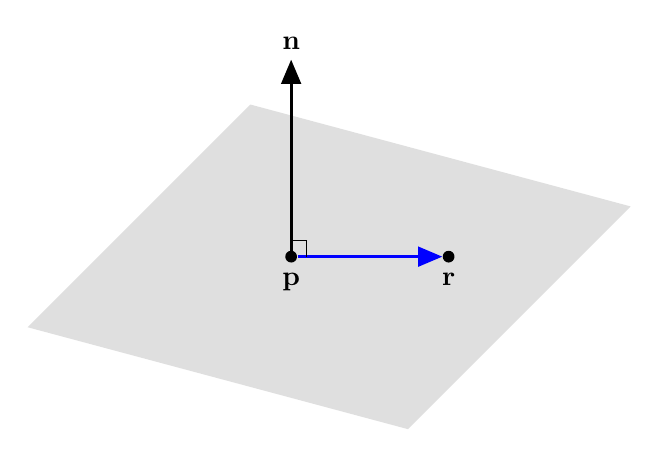
\begin{tikzpicture}
    \tikzmath{\x=-15;\y=45;\z=90;\a=0;}
    \fill [gray!50,opacity=0.5] ($(0,0)+(\x:-1)+(\y:-2)$) -- ++(\x:4) -- ++(\y:4) -- ++(\x:-5) -- ++(\y:-4);
    \node [point,label=below:$\vec{p}$] (p) {};
    \node [point,label=below:$\vec{r}$] (r) at (\a:2) {};
    \draw [vector,black] (0,0) coordinate (1) -- ++(\z:2.5) node [above] {$\vec{n}$};
    \draw [vector] (p) -- (r);
    \draw (\a:0.2) -- ++(\z:0.2) -- ++(\a:-0.2);
\end{tikzpicture}

% Intersecting planes
% \begin{tikzpicture}
%     \draw [blue,fill=blue!20,opacity=0.5] ($(210:1.5)+(150:1.25)$) -- ++(330:2.5) -- ++(30:3) -- ++(150:2.5) -- ++(210:3);
%     \draw [red,fill=red!20,opacity=0.5] ($(150:1.25)+(90:1)$) -- ++(270:2) -- ++(330:2.5) -- ++(90:2) -- ++(150:2.5);
%     \draw [green,fill=green!20,opacity=0.5] ($(210:1.5)+(90:1)$) -- ++(270:2) -- ++(30:3) -- ++(90:2) -- ++(210:3);
%     \draw [opacity=0.5,dashed] (210:1.5) -- ++(30:3) (90:1) -- ++(270:2) (150:1.25) -- ++(330:2.5);
%     \node [point] at (0,0) {};
% \end{tikzpicture}

% \begin{tikzpicture}
%     \draw [green,fill=green!20,opacity=0.5] ($(210:1)+(90:1.25)$) -- ++(270:2.5) -- ++(30:2) -- ++(90:2.5) -- ++(210:2);
%     \draw [blue,fill=blue!20,opacity=0.5] ($(180:1)+(200:1.5)$) -- ++(0:3) -- ++(30:2) -- ++(180:3) -- ++(210:2);
%     \draw [red,fill=red!20,opacity=0.5] ($(210:1)+(150:1.5)$) -- ++(330:3) -- ++(30:2) -- ++(150:3) -- ++(210:2);
%     \draw [opacity=0.5,dashed] (210:1) -- ++(30:2);
% \end{tikzpicture}

% \begin{tikzpicture}
%     \draw [blue,fill=blue!20,opacity=0.5] 
%         ({2.4*cos(30)},{sin(30)}) -- 
%         ({2.4*cos(120)},{sin(120)}) --
%         ({2.4*cos(210)},{sin(210)}) -- 
%         ({2.4*cos(300)},{sin(300)}) -- cycle;
%     \draw [red,fill=red!20,opacity=0.5] 
%         ({2.4*cos(60)},{sin(60)}) -- 
%         ({2.4*cos(160)},{sin(150)}) --
%         ({2.4*cos(240)},{sin(240)}) -- 
%         ({2.4*cos(330)},{sin(330)}) -- cycle;
%     \draw [green,fill=green!20,opacity=0.5] ($(210:1)+(90:1.25)$) -- ++(270:2.5) -- ++(30:2) -- ++(90:2.5) -- ++(210:2);
%     \draw [opacity=0.5,dashed] (210:1) -- ++(30:2);
% \end{tikzpicture}

% \begin{tikzpicture}
%     \draw [green,fill=green!20,opacity=0.5] ($(210:1.25)+(90:1.25)$) -- ++(270:2.5) -- ++(30:2.5) -- ++(90:2.5) -- ++(210:2.5);
%     \draw [blue,fill=blue!20,opacity=0.5] ($(210:1.25)+(150:1.25)+(270:0.5)$) -- ++(330:2.5) -- ++(30:2.5) -- ++(150:2.5) -- ++(210:2.5);
%     \draw [red,fill=red!20,opacity=0.5] ($(210:1.25)+(150:1.25)+(90:0.5)$) -- ++(330:2.5) -- ++(30:2.5) -- ++(150:2.5) -- ++(210:2.5);
%     \draw [opacity=0.5,dashed] ($(210:1.25)+(90:0.5)$) -- ++(30:2.5);
%     \draw [opacity=0.5,dashed] ($(210:1.25)+(270:0.5)$) -- ++(30:2.5);
% \end{tikzpicture}

% \begin{tikzpicture}
%     \draw [green,fill=green!20,opacity=0.5] ($(0:1)+(315:0.5)$) -- ++(30:2.5) -- ++(135:2.5) -- ++(210:2.5) -- ++(315:2.5);
%     \draw [blue,fill=blue!20,opacity=0.5] (180:1.5) -- ++(0:3) -- ++(30:2.5) -- ++(180:3) -- ++(210:2.5);
%     \draw [red,fill=red!20,opacity=0.5] ($(180:1)+(225:0.5)$) -- ++(30:2.5) -- ++(45:2.5) -- ++(210:2.5) -- ++(225:2.5);
%     \draw [opacity=0.5,dashed] (0:1) -- ++(30:2.5);
%     \draw [opacity=0.5,dashed] (90:1) -- ++(30:2.5);
%     \draw [opacity=0.5,dashed] (180:1) -- ++(30:2.5);
% \end{tikzpicture}

% \begin{tikzpicture}
%     \draw [green,fill=green!20,opacity=0.5] (0,0) -- ++(345:3) -- ++(30:2) -- ++(165:3) -- ++(210:2);
%     \draw [blue,fill=blue!20,opacity=0.5] (0,1) -- ++(345:3) -- ++(30:2) -- ++(165:3) -- ++(210:2);
%     \draw [red,fill=red!20,opacity=0.5] (0,2) -- ++(345:3) -- ++(30:2) -- ++(165:3) -- ++(210:2);
% \end{tikzpicture}

% \begin{tikzpicture}
%     \draw [blue,fill=blue!20,opacity=0.5] 
%         ({2.4*cos(30)},{sin(30)}) -- 
%         ({2.4*cos(120)},{sin(120)}) --
%         ({2.4*cos(210)},{sin(210)}) -- 
%         ({2.4*cos(300)},{sin(300)}) -- cycle;
%     \draw [red,fill=red!20,opacity=0.5] 
%         ({2.4*cos(60)},{sin(60)}) -- 
%         ({2.4*cos(160)},{sin(150)}) --
%         ({2.4*cos(240)},{sin(240)}) -- 
%         ({2.4*cos(330)},{sin(330)}) -- cycle;
%     \draw [green,fill=green!20,opacity=0.5] 
%         ({2.4*cos(30)},{sin(30)+2}) -- 
%         ({2.4*cos(120)},{sin(120)+2}) --
%         ({2.4*cos(210)},{sin(210)+2}) -- 
%         ({2.4*cos(300)},{sin(300)+2}) -- cycle;
% \end{tikzpicture}

% \begin{tikzpicture}
%     \draw [green,fill=green!20,opacity=0.5] 
%         ({2.4*cos(0)},{sin(0)}) -- 
%         ({2.4*cos(90)}, {sin(90)}) --
%         ({2.4*cos(180)},{sin(180)}) -- 
%         ({2.4*cos(270)},{sin(270)}) -- cycle;
%     \draw [blue,fill=blue!20,opacity=0.5] 
%         ({2.4*cos(30)},{sin(30)}) -- 
%         ({2.4*cos(120)},{sin(120)}) --
%         ({2.4*cos(210)},{sin(210)}) -- 
%         ({2.4*cos(300)},{sin(300)}) -- cycle;
%     \draw [red,fill=red!20,opacity=0.5] 
%         ({2.4*cos(60)},{sin(60)}) -- 
%         ({2.4*cos(160)},{sin(150)}) --
%         ({2.4*cos(240)},{sin(240)}) -- 
%         ({2.4*cos(330)},{sin(330)}) -- cycle;
% \end{tikzpicture}

% Shortest distance between a point and a line
% \begin{tikzpicture}
%     \tikzmath{\a1=15;\l1=2;}
%     \draw [line width=1pt] (0,0) -- ++(\a1:7) node [pos=0,left] {$\ell$};
%     \node [point,label=below:$\vec{p}$] (p) at (\a1:2) {};
%     \node [green!75!black,point,label=below right:{\color{green!75!black}$\vec{r}=\vec{p} + t\vec{d}$}] (r) at ($(p)+(\a1:3)$) {};
%     \node [point,label=above:$\vec{q}$] (q) at ($(r)+(\a1+90:2)$) {};
%     \draw [vector] (p) -- ++(\a1:2) node [below right,pos=0.5] {$\vec{d}$};
%     \draw [vector,red] (r) -- (q);
%     \draw ($(r)+(\a1+180:0.2)$) -- ++(\a1+90:0.2) -- ++(\a1:0.2);
% \end{tikzpicture}

% Shortest distance between two lines
% \begin{tikzpicture}
%     \coordinate (O1) at (0,0);
%     \coordinate (O2) at (0,3);
%     \coordinate (Q1) at (0,0);
%     \coordinate (Q2) at (0,3);
%     \coordinate (P1) at ($(Q1)+(-1.5,0)$);
%     \coordinate (P2) at ($(Q2)+(160:1.5)$);
%     \draw [green,fill=green!20,opacity=0.3] ($(O1)+(345:-2)+(30:-1.5)$) -- ++(345:4) -- ++(30:3) -- ++(165:4) -- ++(210:3);
%     \draw [blue,fill=blue!20,opacity=0.3] ($(O2)+(345:-2)+(30:-1.5)$) -- ++(345:4) -- ++(30:3) -- ++(165:4) -- ++(210:3);
%     \begin{scope}
%         \clip (1,0) ($(O1)+(345:-2)+(30:-1.5)$) -- ++(345:4) -- ++(30:3) -- ++(165:4) -- ++(210:3);
%         \draw [line width=1pt] ($(O1)+(180:4)$) -- ++(0:8) node [above,pos=0.75,black] {$\ell_1$};
%     \end{scope}
%     \begin{scope}
%         \clip (1,0) ($(O2)+(345:-2)+(30:-1.5)$) -- ++(345:4) -- ++(30:3) -- ++(165:4) -- ++(210:3);
%         \draw [line width=1pt] ($(O2)+(160:4)$) -- ++(340:8) node [above,pos=0.7,black] {$\ell_2$};
%     \end{scope}
%     \node [point,label={270:$\vec{r}_1$}] (q1) at (Q1) {};
%     \node [point,label={90:$\vec{r}_2$}] (q2) at (Q2) {};
%     \node [point,label={270:$\vec{p}_1$}] (p1) at (P1) {};
%     \node [point,label={270:$\vec{p}_2$}] (p2) at (P2) {};
%     \draw (Q1) -- (Q2);
%     \draw ($(Q1)+(0:0.2)$) -- ++(90:0.2) -- ++(0:-0.2);
%     \draw ($(Q2)+(340:-0.2)$) -- ++(270:0.2) -- ++(160:-0.2);
%     \draw [vector, green!75!black] (q1) -- ++(90:1.5) node [left,pos=0.5] {$\hat{\vec{n}}$};
%     \draw [vector, red, line width=1pt] (p1) -- (q1) node [pos=0.5, below] {$\vec{d}_1$};
%     \draw [vector] (p2) -- (q2)node [pos=0.5, above] {$\vec{d}_2$};
% \end{tikzpicture}

% Shortest distance between a point and a plane
% \begin{tikzpicture}
%     \draw [line width=1pt] (0, 0) -- node [pos=0.1,above] {plane} ++(6, 0);
%     \draw [vector] (3, 0) -- ++(90:3) node [left] {$\vec{n}$};
%     \node [point,label={270:$\vec{p}$}] (p) at (3, 0) {};
%     \node [point,label={0:$\vec{q}$}] (q) at (5, 2) {};
%     \draw [vector, red] (p) -- (q);
%     \draw [<->,shorten <= 2pt] (5, 0) -- node [right] {$d$} (q);
%     \draw (3, 2) -- (q);
%     \draw (3,1.8) -- ++(0.2, 0) -- ++(0, 0.2);
%     \draw ($(p)+(45:1)$) arc (45:90:1);
%     \node at ($(p)+(67.5:0.67)$) {$\theta$};
% \end{tikzpicture}

% Subspaces
% \begin{tikzpicture}
%     \draw [fill=blue!10] (0, 0) ellipse (3 and 2);
%     \draw [fill=red!10] (-1, 0) circle (1.5 and 1);
%     \node at (2, 2) {$V$};
%     \node at (0.75, 0.75) {$W$};
%     \node at (-1,0) {$\vec{0}$};
%     \node at (0,0) {$\vec{v}$};
%     \node at (-1,0.5) {$\vec{u}$};
%     \node at (-2,0) {$\alpha \vec{u}$};
%     \node at (-1,-0.5) {$\vec{u} + \vec{v}$};
% \end{tikzpicture}

% Change of basis
% \begin{tikzpicture}
%     \draw [axis] (0, 0) -- ++(0:5) node [right] {$x$};
%     \draw [axis] (0, 0) -- ++(90:4) node [above] {$y$};
%     \draw [vector] (0,0) -- node [below, pos=0.8] {$u_1 \vec{e}_1$} (3,0);
%     \draw [vector] (3,0) -- node [left,pos=0.7] {$u_2 \vec{e}_2$} ++(0,3); 
%     \node [point,label={90:{$u_1\vec{e}_1 + u_2\vec{e}_2 = w_1\vec{v}_1 + w_2\vec{v}_2$}}] (p) at (3, 3) {};
%     \draw [vector,line width=1pt,red] (0,0) -- ++(30:4.1) node [below right,pos=0.9] {$w_1\vec{v}_1$};
%     \draw [vector,line width=1pt,red] (30:4.1) -- (p) node [above right,pos=0.5] {$w_2\vec{v}_2$};
%     \draw [vector,black] (0,0) -- node [below,pos=0.5] {$\vec{e}_1$} ++(0:2);
%     \draw [vector,black] (0,0) -- node [right,pos=0.5] {$\vec{e}_2$} ++(90:2);
%     \draw [vector,black] (0,0) -- node [below right,pos=0.5] {$\vec{v}_1$} ++(30:2) ;
%     \draw [vector,black] (0,0) -- node [below left,pos=0.5] {$\vec{v}_2$} ++(120:2);
% \end{tikzpicture}

% Linear transformation
% \begin{tikzpicture}
%     % \draw [step=0.5, black!20] (-1,-1) grid ++(7, 5);
%     \draw [blue!40] (-1,-1) grid ++(7, 5);
%     \begin{scope}
%         \clip (-1, -1) rectangle ++(7, 5);
%         % \foreach \i in {-5, -4, ..., 5}{
%         %     \draw [blue!40] (2.5 * \i - 0.5, -1) -- ++(5,10);
%         %     \draw [blue!40] (-1, 1.67 * \i - 0.33) -- ++(15,5);
%         % }
%         \foreach \i in {-5, -4, ..., 5}{
%             \draw [red!40] (2.5 * \i - 0.5, -1) -- ++(5,10);
%             \draw [red!40] (-1, 1.67 * \i - 0.33) -- ++(15,5);
%         }
%     \end{scope}
%     \draw [vector,blue,line width=1pt] (0,0) -- node [below] {$\vec{e}_1$} (1,0);
%     \draw [vector,blue,line width=1pt] (0,0) -- node [left] {$\vec{e}_2$} (0,1);
%     \draw [vector,line width=1pt,red] (0,0) -- node [below right,pos=0.67] {$T(\vec{e}_1)$} (3,1);
%     \draw [vector,line width=1pt,red] (0,0) -- node [above left,pos=0.67] {$T(\vec{e}_2)$} (1,2);
%     \fill [red!40,opacity=0.3] (0, 0) -- ++(3, 1) -- ++(1, 2) -- ++(-3, -1) -- cycle;
%     \fill [blue!40,opacity=0.3] (0, 0) rectangle ++(1, 1);
%     \node [point,blue,label={45:\textcolor{blue}{$(1,1)$}}] at (1, 1) {};
%     \node [point,red,label={0:\textcolor{red}{$T\begin{pmatrix} 1\\ 1 \end{pmatrix}$}}] at (4, 3) {};
% \end{tikzpicture}

% Rotation
% \begin{tikzpicture}
%     \tikzmath{\a1=30; \a2=60; \l1=4; \l2=1;}
%     \draw [axis] (0, 0) -- ++(5, 0) node [right] {$x$};
%     \draw [axis] (0, 0) -- ++(0, 4) node [above] {$y$};
%     \node [point, blue] at (\a1:\l1) (1) {};
%     \node [point, red] at (\a2:\l1) (2) {};
%     \draw [vector] (0, 0) -- (1) node [pos=0.75,below] {$\vec{u}$};
%     \draw [vector, red] (0, 0) -- (2) node [pos=0.6,left] {$\vec{v}$};
%     \draw [vector] (0, 0) -- (0:\l1) node [pos=0.6,below] {$\|\vec{u}\|\vec{e}_1$};
%     \draw [vector,black] (0, 0) -- (0:1) node [pos=0.5,below] {$\vec{e}_1$};
%     \draw [-latex'] (\a1:\l2) arc (\a1 : \a2 : \l2);
%     \draw [-latex'] (0:{\l2+0.5}) arc (0 : \a1 : {\l2+0.5});
%     \node at ({0.5 * (\a1+\a2)}: {0.75*\l2}) {$\theta$};
%     \node at ({0.5 * \a1}: {1.2*\l2}) {$\phi$};
%     \draw [blue] (1) -- ({\l1 * cos(\a1)}, 0);
%     \draw [red] (2) -- ({\l1 * cos(\a2)}, 0);
%     \draw [blue] ({\l1 * cos(\a1)-0.2}, 0) -- ++(0, 0.2) -- ++(0.2, 0);
%     \draw [red] ({\l1 * cos(\a2)-0.2}, 0) -- ++(0, 0.2) -- ++(0.2, 0);
% \end{tikzpicture}

% \begin{tikzpicture}
%     \tikzmath{\a1=30; \a2=60; \l1=4; \l2=1;}
%     \draw [axis] (-3, 0) -- (3, 0) node [right] {$x$};
%     \draw [axis] (0, 0) -- ++(0, 3) node [above] {$y$};
%     \node [point,label={0:\textcolor{blue}{$(2,1)$}}, blue] (p) at (26.57:3) {};
%     \draw [vector, blue, line width=1pt] (0,0) -- (p);
%     \node [point,label={180:\textcolor{red}{$(-1,2)$}},red] (q) at (116.56:3) {};
%     \draw [vector,red, line width=1pt] (0,0) -- (q);
%     \draw [-latex'] (26.57:0.75) arc (26.57:116.57:0.75);
%     \node at (71.57:0.5) {$\theta$};
% \end{tikzpicture}

% Reflection
% \begin{tikzpicture}[auto]
%     \tikzmath{\a1=65;\a2=45;\l1=4;}
%     \draw [axis] (0,0) -- (5,0) node [right] {$x$};
%     \draw [axis] (0,0) -- (0,4) node [above] {$y$};
%     \draw [green!75!black,dashed,line width=2pt] (0,0) -- (\a2:\l1+1);
%     \draw [vector] (0,0) -- (\a1:\l1) node [pos=0.5] {$\vec{u}$};
%     \draw [vector,red] (0,0) -- (2*\a2-\a1:\l1) node [pos=0.5,below right] {$\vec{v}$};
%     \draw [dblarrow,shorten >= 2pt] ($(2*\a2-\a1:\l1)+(\a2:0.1)$) -- ++(90+\a2:{\l1*sin(\a1-\a2)}) node [pos=0.5,above right] {$d$};
%     \draw [dblarrow,shorten <= 2pt] ($(\a2:{\l1*cos(\a1-\a2)})+(\a2:0.1)$) -- ++(90+\a2:{\l1*sin(\a1-\a2)}) node [pos=0.5,above right] {$d$};
%     \draw [-latex',bend left,shorten >= 2pt,shorten <= 2pt] (\a1:0.5*\l1) to (2*\a2-\a1:0.5*\l1);
% \end{tikzpicture}

% \begin{tikzpicture}[auto]
%     \tikzmath{\a1=30; \l1=4;}
%     \draw [axis] (0,0) -- ++(5,0) node [right] {$x$};
%     \draw [axis] (0,-2.5) -- ++(0,5) node [above] {$y$};
%     \draw [vector] (0,0) -- (\a1:\l1) node [pos=0.5] {$\vec{u}$};
%     \draw [vector, red] (0,0) -- (-\a1:\l1) node [pos=0.5,below left] {$\vec{v}$};
%     \draw [dashed,green!75!black,line width=2pt] (0,0) -- (\l1+0.5,0);\draw [-latex',bend left,shorten >= 2pt,shorten <= 2pt] (\a1:2) to (-\a1:2);
% \end{tikzpicture}

\tikzmath{\a1=75;\a2=45;\l1=4;}
% \begin{tikzpicture}[auto]
%     \draw [axis] (-1,0) -- ++(6,0) node [right] {$x$};
%     \draw [axis] (0,-2) -- ++(0,6) node [above] {$y$}; 
%     \draw [green!75!black,dashed,line width=2pt,opacity=0.25] (180+\a2:1) -- (\a2:\l1+0.5);
%     \draw [green!75!black,dashed,line width=2pt] (180:1) -- (0:\l1+0.5);
%     \draw [vector,blue!25] (0,0) -- (\a1:\l1) node [pos=0.5] {$\vec{u}$};
%     \draw [vector] (0,0) -- (\a1-\a2:\l1) node [pos=0.5] {$\vec{u}$};
%     \draw [-latex'] (\a2:1) arc (\a2:0:1);
%     \draw [-latex'] (\a1:1.25) arc (\a1:\a1-\a2:1.25);
%     \node at (0.5*\a2:0.67) {$\theta$};
% \end{tikzpicture}

% \begin{tikzpicture}[auto]
%     \draw [axis] (-1,0) -- ++(6,0) node [right] {$x$};
%     \draw [axis] (0,-2) -- ++(0,5) node [above] {$y$};
%     \draw [vector] (0,0) -- (\a1-\a2:\l1) node [pos=0.5] {$\vec{u}$};
%     \draw [vector, red] (0,0) -- (-\a1+\a2:\l1) node [pos=0.5,below left] {$\vec{v}$};
%     \draw [dashed,green!75!black,line width=2pt] (180:1) -- (\l1+0.5,0);
%     \draw [-latex',bend left,shorten >= 2pt,shorten <= 2pt] (\a1-\a2:2) to (2*\a2-\a1-\a2:2);
% \end{tikzpicture}

% \begin{tikzpicture}[auto]
%     \draw [axis] (-1,0) -- ++(6,0) node [right] {$x$};
%     \draw [axis] (0,-2) -- ++(0,6) node [above] {$y$};
%     \draw [vector] (0,0) -- (\a1:\l1) node [pos=0.5] {$\vec{u}$};    
%     \draw [vector, red] (0,0) -- (-\a1+2*\a2:\l1) node [pos=0.5,below right] {$\vec{v}$};
%     \draw [vector, red!25] (0,0) -- (-\a1+\a2:\l1) node [pos=0.5,below left] {$\vec{v}$};
%     \draw [dashed,green!75!black,line width=2pt,opacity=0.25] (180:1) -- (\l1+0.5,0);
%     \draw [dashed,green!75!black,line width=2pt] (180+\a2:1) -- (\a2:\l1+0.5);
%     \draw [-latex'] (0:1) arc (0:\a2:1);
%     \draw [-latex'] (-\a1+\a2:1.25) arc (-\a1+\a2:-\a1+2*\a2:1.25);
%     \node at (0.5*\a2:0.67) {$\theta$};
% \end{tikzpicture}

% \begin{tikzpicture}
%     \draw [axis] (-2,0) -- (4,0) node [right] {$x$};
%     \draw [axis] (0,-2) -- (0,4) node [above] {$y$};
%     \draw [green!75!black,dashed,line width=2pt] (-1,-1) -- (3,3);
%     \draw [vector] (0,0) -- (3,-1) node [below] {$(3,-1)$};
%     \draw [vector,red] (0,0) -- (-1,3) node [above] {$(-1,3)$};
%     \draw (0:1) arc (0:45:1);
%     \node at (22.5:0.67) {$\frac{\pi}{4}$};
% \end{tikzpicture}

% Scaling
% \begin{tikzpicture}
%     \tikzmath{\a1=30;\a2=40;\l1=3;\l2=5;}
%     \draw [axis] (0,0) -- ++(4.5,0) node [right] {$x$};
%     \draw [axis] (0,0) -- ++(0,4) node [above] {$y$};
%     \draw [vector] (0,0) -- ++(\a1:\l1) node [below right,pos=0.5] {$\vec{u}$};
%     \draw [vector, thick, line width=1pt, red] (0,0) -- (\a2:\l2) node [pos=0.5,above left] {$\vec{v}$};
%     \draw [blue,dashed] ({\l1*cos(\a1)},0) -- (\a1:\l1) -- (0,{\l1*sin(\a1)});
%     \draw [red,dashed] ({\l2*cos(\a2)},0) -- (\a2:\l2) -- (0,{\l2*sin(\a2)});
%     \node [blue] at ({\l1*cos(\a1)},0) [below] {$u_1$};
%     \node [blue] at (0,{\l1*sin(\a1)}) [left] {$u_2$};
%     \node [red] at ({\l2*cos(\a2)},0) [below] {$s_1u_1$};
%     \node [red] at (0,{\l2*sin(\a2)}) [left] {$s_2u_2$};
% \end{tikzpicture}

% \begin{tikzpicture}
%     \tikzmath{\x=2;\y=1;\sx=2;\sy=3;}
%     \draw [axis] (0,0) -- ++(5,0) node [right] {$x$};
%     \draw [axis] (0,0) -- ++(0,4) node [above] {$y$};    
%     \draw [vector] (0,0) -- (\x,\y) node [right] {$(\x,\y)$};      
%     \draw [vector, red] (0,0) -- (\sx*\x,\sy*\y) node [right] {$(4, 3)$};
%     \draw [blue,dashed] (\x,0) node [below] {$u_1$} -- (\x, \y) -- (0, \y) node [left] {$u_2$};
%     \draw [red,dashed] (\sx*\x,0) node [below] {$2u_1$} -- (\sx*\x,\sy*\y) -- (0,\sy) node [left] {$3u_2$};
% \end{tikzpicture}

% Translation
% \begin{tikzpicture}[auto]
%     \tikzmath{\a1=20;\a2=50;\l1=4;\l2=4;}
%     \draw [axis] (0,0) -- ++(5,0) node [right] {$x$};
%     \draw [axis] (0,0) -- ++(0,4) node [above] {$y$};
%     \draw [vector] (0,0) -- (\a1:\l1) node [pos=0.5,below right] {$\vec{u}$};
%     \draw [vector,green!75!black] (\a1:\l1) -- (\a2:\l2) node [pos=0.5,above right] {$\vec{t}$};
%     \draw [vector,red] (0,0) -- (\a2:\l2) node [pos=0.5,above left] {$\vec{u} + \vec{t}$};
% \end{tikzpicture}

% \begin{tikzpicture}
%     \tikzmath{\u1=2;\u2=3;\t1=3;\t2=-1;\v1=\u1+\t1;\v2=\u2+\t2;}
%     \draw [axis] (0,0) -- ++(5,0) node [right] {$x$};
%     \draw [axis] (0,0) -- ++(0,4) node [above] {$y$};
%     \draw [vector] (0,0) -- (\u1,\u2) node [pos=0.5,above left] {$(\u1,\u2)$};
%     \draw [vector,green!75!black] (\u1,\u2) -- (\v1,\v2) node [pos=0.5,above right] {$(3,-1)$};
%     \draw [vector, red] (0,0) -- (\v1,\v2) node [pos=0.5,below right] {$(5,2)$};
% \end{tikzpicture}

% Homogeneous co-ordinates
% \begin{tikzpicture}
%     \draw [axis] (-4, 0) -- (4, 0) node [right] {$x$};
%     \draw [axis] (0, -3) -- (0, 5) node [above] {$y$};
%     \coordinate (1) at (-1, -1);
%     \coordinate (2) at (1, -1);
%     \coordinate (3) at (0, 2);
%     \draw [red,line width=1pt, fill=red!20, opacity=0.5] ($2*(1)$) -- ($2*(2)$) -- ($2*(3)$) -- cycle;
%     \draw [blue,line width=1pt,fill=blue!20, opacity=0.5] (1) -- (2) -- (3) -- cycle;
%     \node [point,blue,label={below:\textcolor{blue}{$(-1,-1)$}}] at (1) {};
%     \node [point,blue,label={below:\textcolor{blue}{$(1,-1)$}}] at (2) {};
%     \node [point,blue,label={above:\textcolor{blue}{$(0,2)$}}] at (3) {};
%     \node [point,red,label={below:\textcolor{red}{$(-2,-2)$}}] at (-2, -2) {};
%     \node [point,red,label={below:\textcolor{red}{$(2,-2)$}}] at (2, -2) {};
%     \node [point,red,label={above right:\textcolor{red}{$(0,4)$}}] at (0, 4) {};
% \end{tikzpicture}

% \begin{tikzpicture}
%     \draw [axis] (-4, 0) -- (4, 0) node [right] {$x$};
%     \draw [axis] (0, -4) -- (0, 5) node [above] {$y$};
%     \coordinate (1) at (-2, -2);
%     \coordinate (2) at (2, -2);
%     \coordinate (3) at (0, 4);
%     \coordinate (4) at (0, -2.83);
%     \coordinate (5) at (2.83, 0);
%     \coordinate (6) at (-2.83, 2.83);
%     \draw [blue,line width=1pt,fill=blue!20, opacity=0.5] (1) -- (2) -- (3) -- cycle;
%     \draw [red,line width=1pt,fill=red!20, opacity=0.5] (4) -- (5) -- (6) -- cycle;
%     \node [point,blue,label={below:\textcolor{blue}{$(-2,-2)$}}] at (1) {};
%     \node [point,blue,label={below:\textcolor{blue}{$(2,-2)$}}] at (2) {};
%     \node [point,blue,label={above right:\textcolor{blue}{$(0,4)$}}] at (3) {};
%     \node [point,red,label={below right:\textcolor{red}{$(0,-2\sqrt{2})$}}] at (4) {};
%     \node [point,red,label={above right:\textcolor{red}{$(2\sqrt{2},0)$}}] at (5) {};
%     \node [point,red,label={above:\textcolor{red}{$(-2\sqrt{2},2\sqrt{2})$}}] at (6) {};
% \end{tikzpicture}

% \begin{tikzpicture}
%     \draw [axis] (-4, 0) -- (10, 0) node [right] {$x$};
%     \draw [axis] (0, -4) -- (0, 8) node [above] {$y$};
%     \coordinate (1) at (0, -2.83);
%     \coordinate (2) at (2.83, 0);
%     \coordinate (3) at (-2.83, 2.83);    
%     \coordinate (4) at ($(1)+(6,4)$);
%     \coordinate (5) at ($(2)+(6,4)$);
%     \coordinate (6) at ($(3)+(6,4)$);
%     \draw [blue,line width=1pt,fill=blue!20, opacity=0.5] (1) -- (2) -- (3) -- cycle;
%     \draw [red,line width=1pt,fill=red!20, opacity=0.5] (4) -- (5) -- (6) -- cycle;
%     \node [point,blue,label={below right:\textcolor{blue}{$(0,-2\sqrt{2})$}}] at (1) {};
%     \node [point,blue,label={above right:\textcolor{blue}{$(2\sqrt{2},0)$}}] at (2) {};
%     \node [point,blue,label={above:\textcolor{blue}{$(-2\sqrt{2},2\sqrt{2})$}}] at (3) {};
%     \node [point,red,label={below:\textcolor{red}{$(6, 4 - 2\sqrt{2})$}}] at (4) {};
%     \node [point,red,label={above right:\textcolor{red}{$(6 + 2\sqrt{2},4)$}}] at (5) {};
%     \node [point,red,label={above:\textcolor{red}{$(6-2\sqrt{2},4+2\sqrt{2})$}}] at (6) {};
% \end{tikzpicture}

\end{document}